%!TEX root = ../dissertation.tex

%\begin{savequote}[75mm]
%It is hard for me to empathize with an atom.\footnotemark
%\qauthor{Dr. M. Eric Tai}
%\end{savequote}

\chapter{Optical Lattices and \newline the Bose-Hubbard model}

%\footnotetext{\footnotemark \footnotemark I love my colleague's quote here. Partially because it represents a feeling every AMO graduate student feels at some point, but also because of how close our bonds with atom's should be -- perhaps quite literally.}

\newpage

\section{Single-particle physics in optical lattices}

Ultra-cold neutral atoms in optical lattices provide a new paradigm in the ability to experimentally simulate quantum models. The level of control that can be applied to manipulating atoms enables physicists to realize truly quantum phenomena with level of high precision. In this work, we will ...
T, why they're special and some arguments about deBroglie wavelength. We have very clean systems unlike most real materials. What about when we apply disorder? 

Optical electronic transitions in neutral atoms provide both conservative forces and dissipative forces (metcalf). These two processes can be thought of as elastic and inelastic scattering, respectively, of photons with the atom. The dissipative force is provided by the absorption of a photon or emission of a photo and has been famously used for trapping and cooling of atomic gases. However, the vast majority of all work or models discussed in this thesis will rely on tailoring conservative potentials with almost arbitrary spatial control.  Since the only external forces that interact with the atoms are predominantly conservative, the system remains, to a very good approximation, isolated from the surrounding external environment.

\subsection{Neutral atoms in optical potentials}

A neutral atom experiences a conservative external potentials from optical photons when the light the atom interacts with is far from resonance.  This light, rather than being absorbed by the atom, induces an electric dipole moment in the atom. The amplitude of the alignment, or anti-alignment, of this dipole moment with the external electrical field changes the energy of the atom and is known as the ac-Stark shift. In the case of a two level atom in a monochromatic laser field, where the laser detuning is large enough that the rotating wave approximation can be used, the conservative potential provided by the dipole atom-light interaction is given by: 

\begin{equation}
\label{eqn:Vdipole}
	V_{dipole} (r) \approx \frac{3\pi c^2}{2 \omega_o^3}\frac{\Gamma}{\Delta} I(r)
\end{equation}


where the atomic transition frequency is $\omega_o$, the linewidth of the transition is $\Gamma$, the intensity of the laser power is $I(r)$, and the detuning of the laser frequency from the atomic transition is $\Delta = \omega-\omega_o$. Note that the both the laser intensity, $I(r)$, and the detuning, $\Delta$, are complimentary ways to change dipole potential depth. Additionally, the sign of the detuning $\Delta$ controls whether the atom is attracted to or repelled from the high-intensity locations of the laser beam profile. This is commonly referred to as either red- or blue-detuning of the laser with respect to the atomic transition frequency due to their relationship of the colors in the visible spectrum. While (\ref{eqn:Vdipole}) is written for a two level atom approximation, additional energy levels can be included to provide a more accurate response (cite someone).

However, the laser illuminating the atom does not act purely as a conservative potential since the photons can exchange energy with the the atom by exciting an electron to an excited state. The likelihood of such a dissipative process depends on both the intensity of the light, $I$ and the laser detuning with respect to the linewidth of the atomic transition $\Gamma/\Delta$. The rate at which an atom scatters light is given by (\ref{eqn:gscatter}).

\begin{equation}
\label{eqn:gscatter}
	\Gamma_{sc}(r) \approx \frac{3 \pi c^2}{2 \hbar \omega_o^3} \left ( \frac{\Gamma}{\Delta}  \right )^2 I(r) = \frac{1}{\hbar} \frac{\Gamma}{\Delta} V_{dipole}(r)
\end{equation}

By detuning the laser far from resonance, we see that the scattering rate, or dissipative contribution of the light-atom interaction, is reduced compared to the conservative contribution by a factor of $(\Gamma/\Delta)$. This implies that for the same desired dipole potential depth $V_o$, it is always favorable to increase both the laser detuning and the intensity to reduce the scattering rate to more faithfully realize a purely conservative potential. 

This consideration of these two scalings provide some guidance in how to choose practical parameters for the lasers that produce the desired optical potentials. In the case of $^{87}$Rb, the two relevant optical transitions come from the D1 and D2 lines of the $5s\rightarrow6p$ transition which occur at $\lambda=795$nm and $\lambda=780$nm respectively. All attractive, red-detuned, potentials in this work are derived from a broadband $\lambda\approx840$nm SLED source\footnote{EXALOS bladdy blue}. All repulsive, blue-detuned, potentials are derived from a similar broadband $\lambda\approx758$nm SLED source\footnote{EXALOS bladdy blue2}. We will predominantly study Hamiltonians provided purely by this repulsive light.

\subsection{Bandstructure and Bloch wavefunctions}

All experiments in this thesis will be realized in an effective 1-D optical lattice that is generated from interfering the blue detuned light. The potential generated from this light depends on the intensity of its interference pattern and is written as:

% If, in terms of energy seen by the atom, each beam provides $(V_o/2) e^{\pm i k x - i \omega t}$, then the potential given is by: 

\begin{equation}
\label{eqn:Vpot}
V(x)=-(V_o/2) \cos{\left  (  2 k x \right )}
\end{equation}

where k \footnote{This is k-vector is defined as $2\pi/\lambda$ when the light used to create the potential originates from two counter-propagating lasers where $lambda$ is the laser wavelength. However, this only provides an upper-bound for what k-vector can be produced by a given laser wavelength. What matters is the k-vector in the plane of the lattice formed by the lasers which can be tuned by their relative angle. This point will be further elucidated in Ch.~3.} is the wavevector (or k-vector) of the light used to create the potential and $m$ is the mass of the atom. The potential has been written with no dc-potential offset for convenience. The total Hamiltonian then for a single-particle is written as:
%\begin{equation}
%\label{eqn:lattlight}
% $\left ( (V_o/2) e^{i k x-i \omega t} + (V_o /2) e^{-i  k x - i \omega t})^2 = V_o/2 (e^{i 2 k x} + 2 + e^{- i 2 k x} \right )$
%\end{equation}

\begin{equation}
\label{eqn:HamBS}
H=\frac{\hat{p}^2}{2m}+V(x)
\end{equation}

In the case of zero lattice depth, $V_o$, this Hamiltonian realizes a single-particle in free space whose eigenstates are described by a propagating wave with an eigenenergy that depends only on its momentum $\hbar k$: $\psi_k = e^{i k x/\hbar}$. A side note is that this potential-free Hamiltonian has a continuous spatial translational symmetry and therefore conserves momentum which additionally implies that eigenstates of this Hamiltonian are also eigenstates of the momentum operator $\hat{p}$ \footnote{This is, of course, obvious since the Hamiltonian is composed of only the momentum operator $\hat{p}$. However, the statement about translational symmetry in space and conserved  momentum is a general one and quite powerful.}

Once the lattice depth is non-zero, this symmetry is broken such that the Hamiltonian only retains a discrete translational symmetry. The Bloch theorem states that since the Hamiltonian (\ref{eqn:HamBS}) has a discrete translational symmetry from the periodic potential (\ref{eqn:Vpot}), then the eigenfunctions of the Hamiltonian will also be eigenfunctions of this discrete translation and hence will also be periodic (\ref{eqn:blochFx}).

\begin{equation}
\label{eqn:blochFx}
\phi_q^{(n)} (x) =  e^{i q x/\hbar} \cdot u_q^{(n)}(x)
\end{equation}

The Bloch wavefunctions, $\phi_q^{(n)}$ are labeled by their band index $n$ and their quasi-momentum, or crystal momentum, $q$. This quasi-momentum is akin to the linear momentum of the free-particle case referenced to above except that it is now only defined within the Brillouin zone of the periodic potential $- \hbar k_L \leq q \leq \hbar k_{L}$ where $k_L$ is the k-vector of the lattice. The function $u_q^{(n)}(x)$ is a Fourier series with a periodicity that correspond to multiples of the lattice period. Intuitively, this high-frequency cut off when $q=\pm k_L$.

To find the eigenfunctions of this new Hamiltonian with momentum states coupled by multiples of twice the lattice period, we can more conveniently solve this problem in Fourier space and solve for the eigenergies $E_q^{(n)}$. We first write both the potential and the periodic function $u_q^{(n)}(x)$ as Fourier series:

\begin{equation}
\label{eqn:FSV}
V(x) = \sum_m V_m e^{i  2 m k x}
\end{equation}

and

\begin{equation}
\label{eqn:ux}
u^{(n)}(x) = \sum_l c_l^{(n,q)} e^{i 2 l k x}
\end{equation}

The periodic potential term $V(x)$ in (\ref{eqn:FSV}) only has two non-zero terms that correspond to the lattice periodicity $ \left ( V_{m=-1} = V_{m=1} = -V_o / 4 \right ) $. To find the coefficients for the Fourier series of $u_q^{(n)}$ and the eigenenergies $E_q^{(n)}$ one should exploit the orthogonality relation between Fourier modes after taking the inner-product  of $\langle e^{i 2 l' k x} | H | \phi_q^{(n)} \rangle$ (please refer to Appendix \ref{appendix:Ch1Cal}. This procedure results in:

\begin{equation}
\label{eqn:HamC}
\sum_l' H_{l,l'} \cdot c_l^{(n,q)} = E_q^{(n)} c_l^{(n,q)}
\end{equation}

where

\begin{equation}
\label{eqn:HamLL}
H_{l,l'} = \left \{
\begin{array}{ll}
      (2 l + q / k)^2 ,& l=l' \\
      -V_o/4, & | l-l' | = 1 x \\
\end{array} 
\right .
\end{equation}

Diagonalizing the Hamiltonian (\ref{eqn:HamLL}), where $l$ and $l'$ are matrix indices, will solve for the eigenenergies that depend on the continuous variable $q$ and the discrete index $n$ which labels the characteristic formation of \emph{bands} in the spectrum. To gain some intuition for the system this Hamiltonian describes, we can first think about the $V_o=0$ case. In the case of no external potential, this Hamiltonian will realize a parabolic dispersion curve in $k$-space from the momentum of a free-particle. By turning on the lattice potential $V_o \neq 0 $ the external potential can now provide momentum kicks to the particle's wavefunction in discrete quant of $2\hbar k$ (when the indices $l,l'$ differ by $1$). In the case that the energy from the free-particle dispersion curve at  $q$ and $q\pm 2\hbar k$ are $\lesssim V_o$, then these two momentum states are strongly coupled and these states hybridize to make form an eigenstate. The first happens is at the $q=\hbar k$ point in the dispersion curve and defines what is know as the Brillouin zone boundary in a crystal. Physically, this hybridization corresponds to perfect Bragg reflection of the particle's wave function at the Brillouin zone boundary. This hybridization forms the familiar \emph{gaps} associated between bands of energy as defined on a reduced Brillouin zone band diagram (\ref{fig:freePartBS}).

\begin{figure}[ht!]
		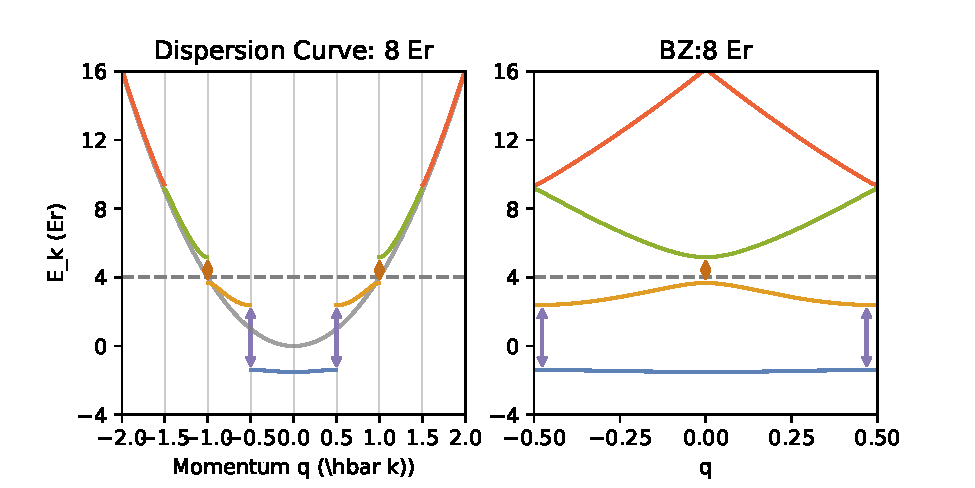
\includegraphics[width=\columnwidth]{figures/ch1/BandStructure/BZ_BS.pdf} 
		\caption{\textbf{Dispersion with Bragg reflection. a,}  The left curve shows free-particle dispersion parabola + gaps opening up from Bragg scattering off the lattice. Additionally, the dashed-grey lines show the height of the lattice as it is centered about zero and determines when a state $| \psi_k^{(n)} \rangle$ is bound to the lattice. In this case ...  This depiction of the hybridization of the free-particle dispersion curve is known as the extended Brillouin zone scheme and is an intuitive way of how to reach the notion of bands from Bragg scattering.  \textbf{b} depicts the more familiar reduced Brillouin zone scheme associated with condensed matter physics and band structure. This mapping is both compact and conceptually reflects the notion of periodic states that are described by Bloch wavefunctions $| \phi_q^{(n)} \rangle$ that are only well defined for quasi-momentum states $q$ that are bounded by the lattice wave-vector $k_L$.}
		\label{fig:freePartBS}	
\end{figure}

Once the lattice depth, $V_o$, is deep enough that an entire band lies within its energy window, it conceptually makes sense to describe these as Bloch functions that are bound to the lattice and are the free-particle states dressed by free-particle states with integer multiples of the lattice vector $2\hbar k$. This is shown for both the ground band and the first excited band in in Fig.~\ref{fig:freePartBS}. This thesis will use the convention that $n=0$ refers to the ground-band. These periodic eigenstates of the Hamiltonian are plotted for various quasi-momentum states for both the ground band and the excited band in Fig.~\ref{fig:blochFx}.  A common physical picture given for the opening of a gap at the edge of the Brillouin zone is given by the phase of the Bloch wavefunction's spatial structure. While $| \phi_{q=\hbar k}^{n=0,1} (x) \rangle \approx e^{i k x} + (-1)^n e^{-i k x}$  are both composed of the same free-particle momenta states, their symmetric versus anti-symmetric superposition either concentrates the density of the particle either in the minima or the maxima of the lattice potential (as shown in Fig.~\ref{fig:blochFX}).

\begin{figure}[ht!]
		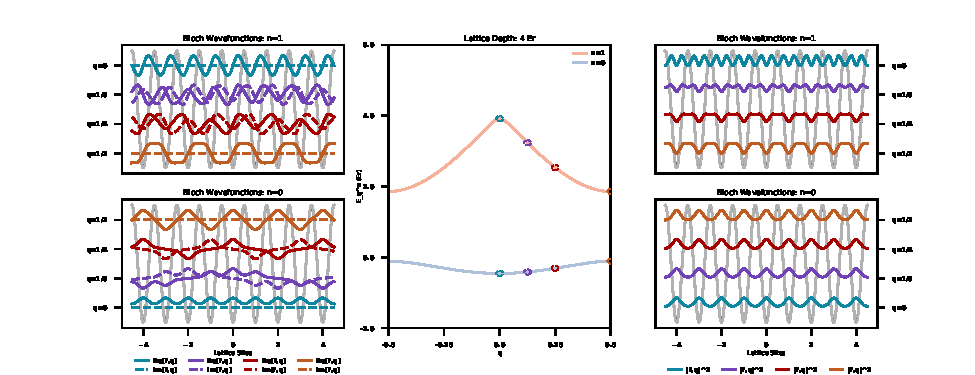
\includegraphics[width=\columnwidth]{figures/ch1/blochFx/BlochFunctionsBS2.pdf} 
		\caption{\textbf{Bloch wavefunctions. a,} The left plots depict the real and imaginary parts of the Bloch wavefunction's ($ | \phi_q^{(n)} (x) \rangle$) spatial dependence as a function of distance for various quasi-momenta and both the $n=0$ and $n=1$ bands at a lattice depth of $4E_r$. \textbf{b} Plots the band structure for at $4E_r$ and the quasi-momenta  the plotted Bloch wavefunctions describe. \textbf{c} These right plots depict the density distribution of the Bloch functions for the same quasi-momenta as the left plots and same bands. Note that the ground-band, $n=0$, is well bound to the lattice and relatively "flat". This qualitatively means that the distribution of the ... for both a and c describe that the periodicity is basically the same, in the deep limit it is only the phase that appreciably changes.. Something something cosine dispersion.}
		\label{fig:blochFX}	
\end{figure}

There are two primary quantities that are typically extracted from the band structure due to their physical relevance: the band width and the band gap. The band width, the energy difference between the maximum and minimum energy for a given band ($arg \max_q {\left \{ E_q^{(n)}  \right \}}- arg \min_q { \left \{ E_q^{(n)} \right \} })$, describes the maximum kinetic energy of a particle in that band. The kinetic energy becomes substantially suppressed as bands become bound to the lattice and will appear as approximately flat. The band gap, the energy difference between successive bands $\Delta = E_q^{(n+1)} - E_q'^{(n)} $ defines how well separated a particle in one band is energetically from another band. Practically speaking, all the physics in this thesis will assume a single-band model where all particles inhabit  the ground-band of the lattice. This makes the band gap a relevant metric for determining how well the observed phenomena will be described by a single-band and how susceptible the system will be some form of heating that will deposit energy into the system. The evolution of the band gap and band width can be seen from progression of band structure plots in Fig.~\ref{fig:bandGaps} as well as the evolution of the band gaps between various successive bands as a function of lattice depth.

\begin{figure}[h!]
		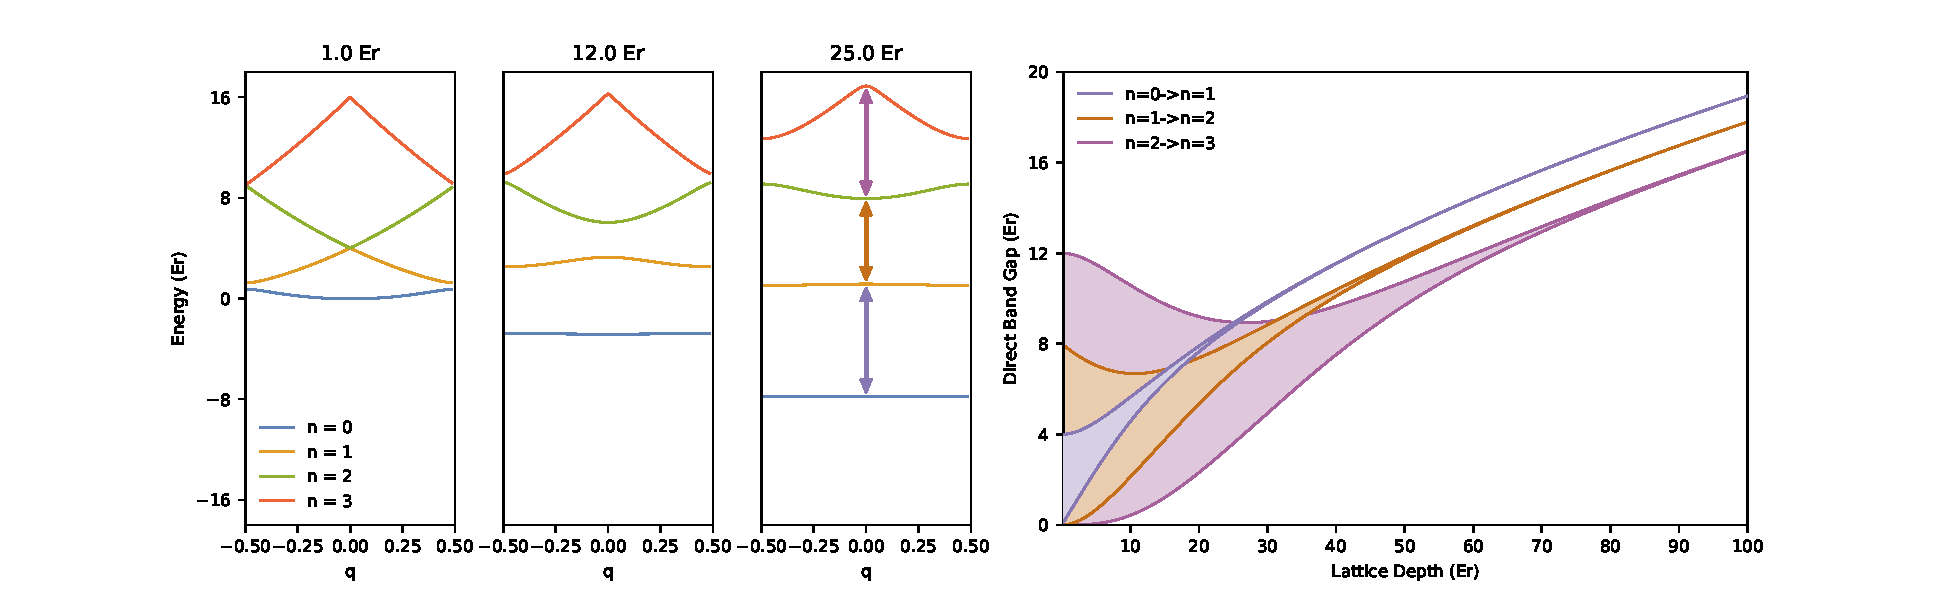
\includegraphics[width=\columnwidth]{figures/ch1/BandStructure/BSScale.pdf} 
		\caption{\textbf{Band Gaps. a,} The band structure of the four lowest bands are plotted for three lattice depths to depict how both the band widths and band gaps change as a function of lattice depth. Note that the lower bands both flatten and become gapped from the excited bands more quickly as a function of lattice depth. \textbf{b,} The band gap between successive bands can strongly depend on which quasi-momentum is being excited from and to ($\Delta_{q,q'}^{n,n+1}=E_q^{(n)}\rightarrow_{q'}^{(n+1)}$). In principle both direct, quasi-momentum preserving, and indirect, non quasi-momentum preserving, excitations are possible in a lattice. However, in the case of a simple sinusoidal lattice, both the minimum and maximum band gaps are captured by just analyzing direct band excitations. The minimum and maximum band gaps are plotted as the solid lines and the distribution of all intermediate possible values are plotted as the shading.}
		\label{fig:bandGaps}	
\end{figure}

\subsection{Wannier wavefunctions}

The Bloch wavefunctions, as the single-particle eigenstates, are a convenient way to describe the physics of a particle in a periodic potential. They are a complete set of energy eigenstates and completely described by their band index n an quasi-momentum q. Since they are defined by a single quasi-momentum number q, they are maximally localized in momentum space and maximally delocalized in position space. An useful alternative, orthonormal basis for this system is given by the set of functions that describe the particle as localized in position space. These set of functions are known as Wannier functions and are a convenient way to describe the wavefunction of a particle in a band $n$ that is maximally localized at a lattice site $x_i$. This basis can be constructed from a superposition of all Bloch wavefunctions   within the Brillouin zone for a given band n:

\begin{equation}
w_n(x-x_i) = \frac{1}{\mathcal{N}} \sum_q e^{-i q x_i} \phi_q^{(n)} (x)
\label{eqn:wnfx}
\end{equation}.

The normalization factor $N$ depends on the finite number of quasi-momentum Bloch wavefunctions summed over. There are some additional subtleties that revolve around practically constructing these functions numerically and are elucidated in more detail in Appendix \ref{appendix:Ch1Cal}. Additionally, since the Bloch wavefunctions are eigenstates of the original Hamiltonian, they may have been solved with an arbitrary global phase that will become an important relative phase in the construction of the Wannier functions $w_n(x-x_i)$.  Thankfully, there is a convenient recipe to follow that establishes how to choose the phases when constructing $w_n(x-x_i)$ that produces a wavefunction maximally localized on site $x_i$.

We have seen from the symmetry of the periodic potential, the hybridization of the free-particle states at the edge of the Brillouin zone, and the plots of the Bloch functions in Fig.~\ref{fig:blochFX} that the wavefunctions of even bands ($ n = 2\times m, m\in  \mathbb{Z}$) are also even functions of $x$ and the wavefunctions of odd bands are also odd functions of $x$. The Wannier functions will also retain this symmetry since they are constructed from the Bloch functions within a given band. To then construct a maximally localized wavefunction at lattice site $x_i$, we must find the necessary phases multiplied by the Bloch wavefunctions that constructively add at $x=x_i$. For even bands, this we a phase for each Bloch function that makes it both real and positive at $x=x_i$. \footnote{It doesn't actually matter which phase you pick for this site, just that you rotate all Bloch wavefunctions such that their phase is the same at $x=x_i$ : $Arg \left [  \phi_q^{(n)} \right ] = const.$ $\forall$ $q$ where $const. \in \mathbb{C}$} For odd bands, the Bloch wavefunctions are also odd about the center of each lattice site $x=x_i$. The recipe used above is modified such that the phase chosen is such that the first derivative of the Bloch wavefunctions are real and positive at site $x_i$. Including the recipes described above we can write down the Wannier functions construction as follows:

%$(Arg \left [ \phi_q^{(n)}(x) |_{x=x_i}  \right ] = const.)$.
%$(Arg \left [ \partial \phi_q^{(n)}(x)/dx |_{x=x_i}  \right ] = const)$

\begin{equation}
\label{eqn:wFx}
w_n(x-x_i) = \left \{
\begin{array}{ll}
     \frac{1}{\mathcal{N}} \sum_q  e^{\left (  - i Arg [ \phi_q^{(n)} (x_i) ] \right )} \cdot \phi_q^{(n)} (x), & n\mathrm{\text{ is even}}\\
      \frac{1}{\mathcal{N}} \sum_q  e^{\left (  - i Arg [ \partial \phi_q^{(n)} (x)/ \partial x |_{x=x_i} ] \right )} \cdot \phi_q^{(n)} (x), & n \mathrm{\text{ is odd}}\\
\end{array} 
\right .
\end{equation}

The Wannier wavefunctions represent the maximally localized, conjugate basis to the Bloch wavefunctions. These Wannier states become more localized for increasing lattice depth, which is plotted in Fig.~\ref{fig:wFx}a for the ground band. We can see additionally see plotted in Fig.~\ref{fig:wFx} for a 45$E_r$ lattice how the Wannier wavefunctions are also successively wider for higher bands in the lattice. 

\begin{figure}[ht!]
		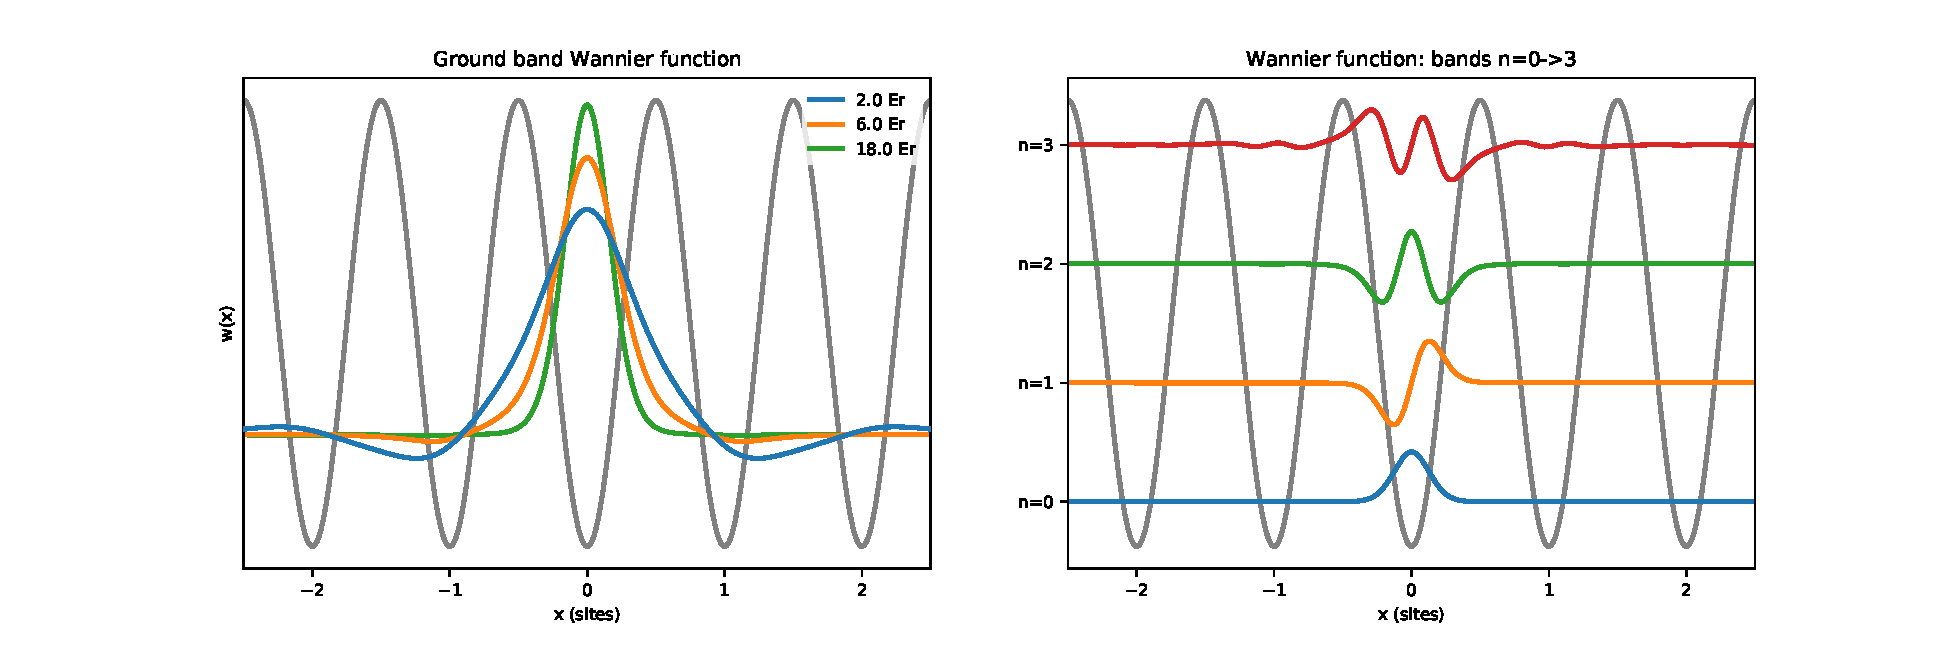
\includegraphics[width=\columnwidth]{figures/ch1/BHParams/WannierFx.pdf} 
		\caption{\textbf{Wannier wavefunctions. a,}  .}
		\label{fig:wFx}	
\end{figure}

A few useful observations can also be made from both the analytical form of $w_n(x-x_i)$ (\ref{eqn:wFx}), the bands from which they are constructed (Fig.~\ref{fig:freePartBS}) that coincide with their plots in Fig.~\ref{fig:wFx}. Since successively higher bands are mapped from a higher, but limited range, of free particle momenta, we see that $w_n(x-x_i)$ must contain only Fourier components that correspond to the range $n \cdot \hbar k_L \leq k \leq (n+1) \cdot \hbar k_L$. Hence, the Wannier functions for successively higher bands, while still maximally localized, contain a corresponding wrapping of the wavefunction by $n \cot \pi$. Additionally, as the lattice depth becomes much larger than the band width of a given band, the Wannier functions approach the wavefunctions of a Harmonic oscillator, as can be seen by the similarity between the similarity between the $w_n(x-x_i)$ plotted in Fig.~\ref{fig:wFx}b and Hermite Gaussians.\footnote{This is additionally a conceptually comforting fact as the cosine potential providing the lattice can be approximated to lowest order as a quadratic potential. However, due to the finite depth of the lattice, there is always a non-negligible amplitude in the wings of $w_n(x-x_i)$ that is necessary for an accurate description of the system} Lastly, while the Wannier functions are not eigenstates of the original Hamiltonian, they become asymptotically close as $V_o \rightarrow \infty$, where both the corresponding band becomes flatter and the associated Bloch wavefunctions will be nearly degenerate.

\section{The Bose-Hubbard model}

The treatment for deriving band structure and Bloch wavefunctions describe the entire physical story for a single-atom in an optical lattice. However, it neglects the many-body physics associated with interacting particles that leads to celebrated exotic condensed matter systems. It additionally does not easily lend itself to describing the nature of inter-particle interactions that are often derived from a local, inter-particle potential. To incorporate these local dependencies, we will now reformulate the free-particle Hamiltonian from before into a local basis that utilizes our derivation of the Wannier functions in the previous section.

In particular, we will describe the overlap of an atom's wavefunction with a local Wannier function defined about a particular lattice site as the population of the atom in an orbital about that site. This leads us towards adopting the tight-binding lattice model for bosonic particles that is known as the Bose-Hubbard model. This is a renowned toy condensed matter model that faithfully incorporates strong inter-atomic interactions that lead to strongly correlated states that are otherwise absent in interaction corrected mean-field equations, such as the Gross-Pitaevski equation (ref someone besides Philipp, Jacksch et al). 

\subsection{Interacting atoms in an optical lattice}

In all our experiments, we work with dilute atomic gases. In these dilute gas regimes, the atom-atom interactions can be described be an effective inter-atomic potential between any two particles  $V(\textbf{r}$, where $\textbf{r}$ is the inter-particle distance. This potential is strongly repulsive at distances on the order of a few Bohr radii, $(\sim a_o)$, due to the strong Coulomb interaction between the respective atom electron clouds. However, since atoms are polarizable, they are attractive at long distances due to the mutually induced dipoles that lead to a van der Walls force (ref rma 26). 

In the case of low temperature regime utilized by ultracold atom experiments, these inter-atomic interactions primarily result in elastic scattering processes between the atoms. In this regime, it isn't necessary to know the exact shape of the interatomic potential since the low kinetic energies of the atoms do not enable them to probe past the centrifugal barrier. This means that only the lowest partial wave scattering process, \emph{s}-wave scattering, significantly contributes to the inter-atomic interactions.  Therefore, this contribution can be well approximated by a contact interaction that is characterized by a single parameter that quantifies the \emph{s}-wave scattering length, $a_s$: 

\begin{equation}
\label{eqn:UCPot}
V(\textbf{r})=\frac{4 \pi \hbar^2 a_s}{m} \delta (\textbf{r})
\end{equation}

They are often tunable (ma citation 12) via Feshbach resonances where the interaction strength can be changed by many orders of magnitude and even change sign. Unitary limit. We determine our interaction strength via the lattice depth \footnote{Explain $^{87}$Rb problem for Feshbach resonances}.

\subsection{Deriving the Bose-Hubbard model parameters}

We can derive the Bose-Hubbard model by incorporating the inter-atomic contact interactions into the Hamiltonian of a bosonic field $\hat{\Psi}(x)$ and an external potential:

\begin{equation}
\label{eqn:BHHL}
%\begin{multline*}
H =  \int d^3 x~\hat{\Psi}^\dagger (x) \left ( -\frac{\hbar^2}{2m} \nabla^2 + V(x) \right ) \hat{\Psi}(x) ~+ \frac{1}{2} \frac{4 \pi \hbar^2 a_s}{m} \int d^3 x \int d^3 x' ~\hat{\Psi}^\dagger (x) \hat{\Psi}^\dagger (x') \delta(x-x') \hat{\Psi} (x) \hat{\Psi} (x')
%\end{multline*}
\end{equation}

Here the potential contains both the lattice potential and any additional potential term applied on top of the lattice that is relatively weak and spatially varies more slowly than the lattice itself: $V(x)=V_{latt}(x) + V_{arb}(x)$. In the low temperature regime, the atoms only populate the ground band and we can restrict this derivation to involving only basis states that overlap with this band. Since the interaction term is entirely local it is convenient to expand the bosonic field $\hat{\Psi}(x)$ in terms of ground band Wannier wavefunctions:

\begin{equation}
\label{eqn:wfh}
\hat{\Psi}(x) = \frac{1}{\mathcal{N}} \sum_i \hat{a}_i w_o(x-x_i)
\end{equation}

Here $\hat{a}_i$ $(\hat{a}^\dagger_i)$ are the annihilation (creation) operators for a boson in the ground band Wannier function cetreed at a lattice site $x_i$. These operators follow the typical bosonic commutation relation  $  [\hat{a}_i, \hat{a}_j^\dagger]=\delta_{i,j}$. This expansion allows us to rewrite $\ref{eqn:BHHL}$ in terms of these bosonic annihilation and creation operators:

\begin{equation}
\label{eqn:BHM}
H= - \sum_{i,j} J_{i,j} \hat{a}_i^\dagger \hat{a}_j + \sum_{i,j,k,l} \frac{U_{i,j,k,l}}{2} \hat{a}_i^\dagger \hat{a}_j^\dagger \hat{a}_k \hat{a}_l + \sum_i (h_i - \mu) \hat{a}^\dagger_i \hat{a}
\end{equation}

The additional potential that was added on top of the lattice, $V_{arb}(x)$, provides a variation in the on-site energy potential $h_i$. The chemical potential $\mu$ is a thermodynamic quantity that constraints the total particle number  in the grand canonical ensemble description of the model.  The $J_{i,j}$ term is known as the tunneling matrix element quantifies the tunneling rate between any two sites $i$ and $j$ and describes the kinetic energy of the atom. The $U_{i,j,k,l}$ term describes the various interaction matrix elements between atoms on sites $i,j,k,l$.  Although the Wannier functions are all orthognoal, they were never eigenstates of the original Hamiltonian. Formally then, we can quantify these matrix elements via the overlap of the Wannier function after the Hamiltonian has acted on them: 

\begin{equation}
J_{i,j} = - \int d^3 x ~ w^*_0 (x-x_i) \left ( - \frac{\hbar^2}{2m} \nabla^2 + V_{latt}(x) \right ) w_0(x-x_j) 
\label{eqn:J}
\end{equation}

\begin{equation}
U_{i,j,k,l} = \frac{4 \pi \hbar^2 a_s}{m} \int d^3 x ~  w^*_0 (x-x_i)  w^*_0 (x-x_j) w_0(x-x_k) w_0(x-x_l)
\label{eqn:U}
\end{equation}

For nearly all practical cases, we will work in the ``tight-binding" regime of this ground band model. This approximation assumes that the Wannier functions are sufficiently localized that all higher order tunneling processes and higher order interaction terms may be ignored. This leave the model with only a nearest-neighbor tunneling $J_{i,i\pm1}\equiv J$ and on-site interaction $U_{0,0,0,0}]\equiv U$ and results in the stand form of the celebrated Bose-Hubbard model:

\begin{equation}
H_{BH} = - J \sum_{\langle i,j \rangle} \hat{a}^\dagger_i \hat{a}_j + \frac{U}{2} \sum_i \hat{n}_i (\hat{n}_i-1) + \sum_i (h_i - \mu) \hat{n}_i
\label{eqn:BHC}
\end{equation}

where $\hat{n}_i = \hat{a}_i^\dagger \hat{a}$ is the on-site number operator and the bracket sum, $\langle i,j \rangle$ refers to a sum only over neighboring indices. Physically, the mechanism that describes the exact contributions for the on-site interaction term comes from the sum of all pair-wise interactions of $n$ atoms on site $i$, each of which contribute an energy cost of $U$ : $U \sum_i {\hat{n}_i \choose 2}  = U \sum_i \frac{\hat{n}_i!}{(\hat{n}_i-2)! 2!} $.


Both parameters J and U change significantly as a function of the lattice depth $V_o$. The qualitative features of the states that are harbored by the Bose-Hubbard model depend only on the ratio of these two quantities $U/J$. Practically speaking, the absolute energy scales of these two parameters are important for defining relevant experimental time-scales. This conversion comes from defining all energies by $\hbar$ as an \emph{angular} frequency. In our experiment, the depth of the lattice is measured in lattice recoil $E_r/\hbar \approx 2\pi \times 1240 \mathrm{Hz}$ and sets these overall energy scales. The values for J and U, as calculated from the ground state Wannier wavefunctions (\ref{eqn:J}, \ref{eqn:U}), are plotted for the parameters of our experimental parameters in Fig.~\ref{fig:BHP}. 

\begin{figure}[ht!]
		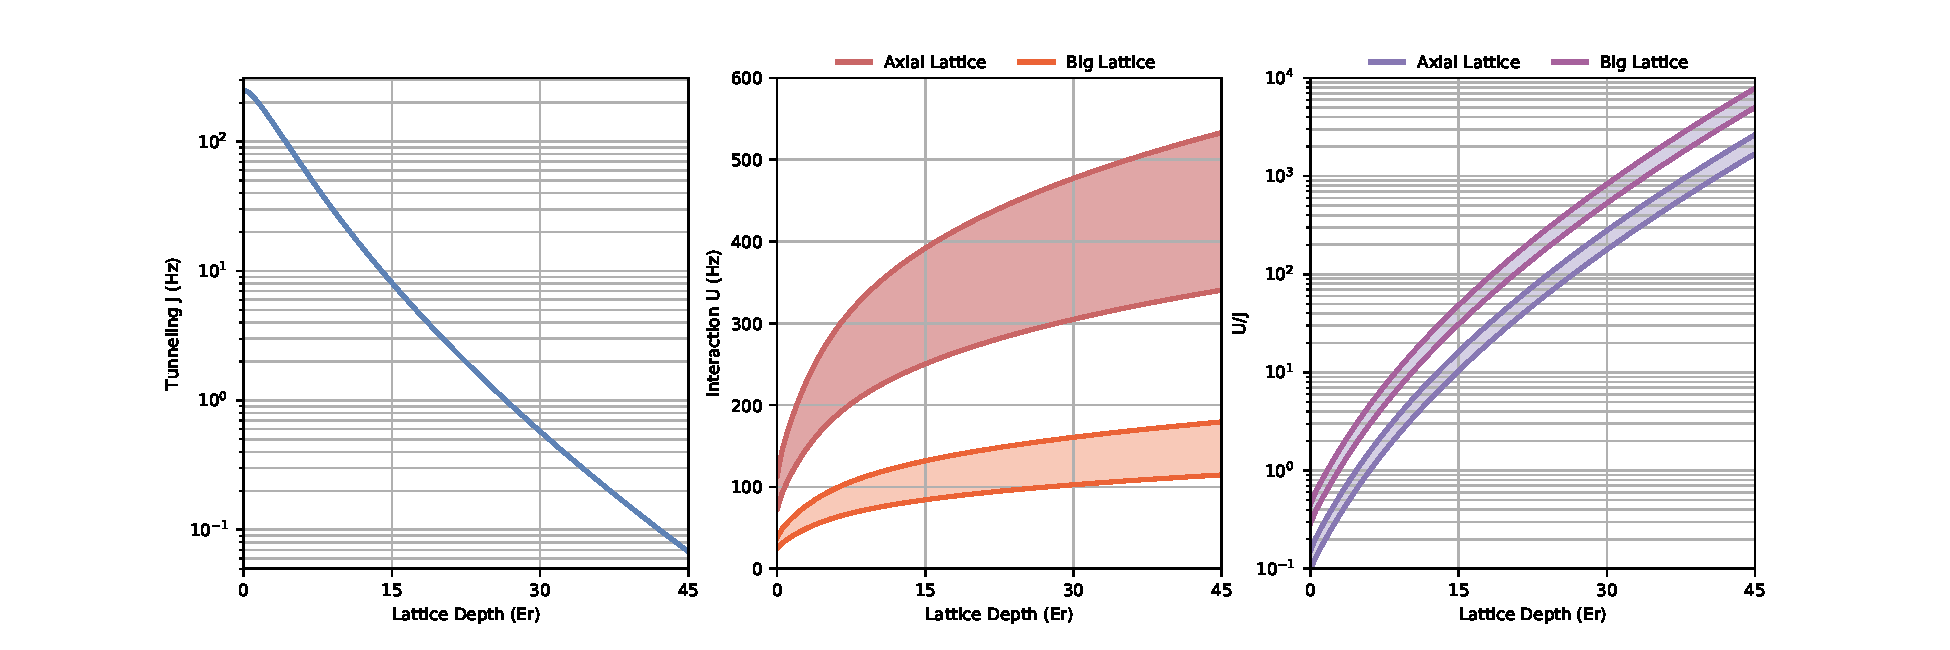
\includegraphics[width=\columnwidth]{figures/ch1/BHParams/BHParams.pdf} 
		\caption{\textbf{Bose-Hubbard Parameters. a,}  All plotted for a 1-D Lattice.}
		\label{fig:BHP}	
\end{figure}

In the deep lattice (tight-binding) limit, the dispersion of the ground band becomes well approximated by a cosine potential, $E_q = - 2 J \cos{\left (2 \pi q/k_L \right )}$ where $J$ is the Bose-Hubbard hopping parameter. In this regime can be solved for exactly and approximately decays exponentially with lattice depth:

\begin{equation}
\label{eqn:tightJ}
J = \frac{4}{\sqrt{\pi}} E_r \left ( \frac{V_o}{E_r}  \right )^{3/4} e^{-2 (V_o/E_r)^{1/2}}
\end{equation}

 Additionally, the scaling of $U$ with lattice depth can be estimated by approximating Wannier wavefunctions with the Harmonic Oscillator Gaussian states. In this limit the two relevant comparisons to the lattice can be given by the effective on-site trap frequency $\omega_{ho}$ and oscillator length $l_{ho}$ that depend on the lattice depth:
 
\begin{equation}
\label{eqn:w_ho}
\omega_{ho} = 2 E_r \sqrt{V_o/ E_r}
\end{equation}

\begin{equation}
\label{eqn:l_ho}
l_{ho}=\sqrt{\hbar / m \omega_{ho}} = \frac{a/2}{2\pi} \left ( \frac{V_o}{E_r} \right )^{-1/4}
\end{equation}

\begin{equation}
\label{eqn:wnHO}
w_n(x-x_i) \approx \psi_{l_{ho}}^n = \frac{1}{\sqrt{2^n n!}} \left ( \frac{1}{\pi l_{ho}^2} \right )^{1/4} e^{-x^2/(2 l_{ho}^2)} H_n (x / l_{ho})
\end{equation}

where $H_n(x/l_{ho})$ are the Hermite polynomials of order $n$.

	This leads to an approximate scaling of $U\propto V_o^{1/4}$. This elucidates the point that while both $J$ and $U$ are tunable with lattice depth, the relevant ratio of $U/J$ is mostly determined by the exponential suppression of $J$ with the lattice depth. However, one difference is that $J$ depends only on the lattice depth along the direction it defines tunneling. This is not the case for $U$ which is nonlinear and depends on the integral of the Wannier wavefunction in all three dimensions. This means that even without using a Feshbach resonance, there is some marginal tunability of $U$  by just changing the lattice depth in the dimensions orthogonal to the dimension of interest. This is particularly relevant since the majority of the work described in this thesis is performed for one dimension. The lattices that provides confinement along the $z$-direction has the widest range of tunability and is plotted in Fig.~\ref{fig:BHP} as two-bands of experimentally accessible ranges.

%Intuitively it then makes sense that the time evolution operator from this Hamiltonian acting on any Wannier function will now inherently break this orthogonality.

%we are using second quantization

\section{Quantum phase transitions: superfluid to Mott-insulator}

Quantum phase are a celebrated achievement in physics that differ from their classical counterparts since they can occur even at zero temperature. These quantum phase transitions are driven by quantum fluctuations in the ground state wavefunction of a system since all thermal fluctuations are frozen out at zero temperature. The Bose Hubbard model famously exhibit two distinct quantum phases that depend on the relative strengths of the on-site interaction and tunneling terms. This will first be described by the ground state wavefunctions behavior in the two extremes for a lattice with no additional potentials, $h_i = 0$, $N$ atoms, and periodic boundary conditions.

\subsection{Superfluid phase: $J \gg U$}

In the limit of very large $J$ compared to $U$, the Hamiltonian favors the delocalization across the lattice. The ground state wavefunction becomes simple to write down in the extreme case that $U\rightarrow0$ and we recover atoms occupying the Bloch band for $q=0$ as defined from the band structure derived earlier in this chapter: 

\begin{equation}
\label{eqn:SF}
| \Psi_{SF} \rangle = \frac{1}{N} \left ( \hat{a}^\dagger_{q=0} \right )^N |0\rangle \propto \frac{1}{N} \left (\sum_i \hat{a}^\dagger_i \right )^N |0\rangle
\end{equation} 

where $|0\rangle$ is defined as the vacuum state with 0 bosons. In the case that we don't restrict the ground state to a specific number of particles $N$, the ground state is defined by a coherent state $|\alpha_i\rangle$ on every site $i$ since this state is an eigenstate of the tunneling matrix elements $\hat{a}_i$. In this regime of uncertain particle number the ground state becomes a product state of coherent states:

\begin{equation}
\label{eqn:SFcoh}
|\Psi_{SF} \rangle \approx \prod_i |\alpha_i\rangle = \prod_i e^{- |\alpha_i |^2 /2} e^{\alpha \hat{a}^\dagger_i} |0\rangle
\end{equation}

where the phase of $\alpha$ is well defined and constant across all sites in the lattice ($\hat{\phi} |\alpha_i\rangle = Arg[\alpha_i]$) and a fixed average density $\langle n \rangle = | \alpha |^2 $. This approximation conceptually describes the superfluid as an array of Bose-Einstein condensates on each lattice site with a well defined phase locked across the entire lattice via the tunneling term. The superfluid phase is defined by a non-zero order parameter $\psi \equiv \langle \alpha \rangle$ and has characteristic properties of having gapless excitations and finite compressibility $\kappa = \partial n/\partial \mu$.

\subsection{Mott-insulator: $U \gg J$}

In the opposite limit, as $U$ becomes the dominant energy scale in the system, the eigenstates of the ground state become defined by the on-site atom number. This forms an insulating state that suppresses particle transport due to the strong inter-atom interactions. This becomes clear in the extreme limit as $J\rightarrow 0$ and the Hamiltonian is now defined by only the on-site number operator $\hat{n}_i$ meaning that all the eigenstates of the Hamiltonian are also eigenstates of $\hat{n}_i$.  Since the on-site particle number is quantized, the atom-number on a given site $i$ is determined by the ratio of $\mu/U$. In the case of a commensurate total atom number $N$ with the number of lattice sites ($N/L=n$), the Mott-insulator wavefunction is written as:

\begin{equation}
\label{eqn:MI}
|\Psi_{MI}\rangle = \prod_i \left ( \hat{a}_i^\dagger \right )^n |0\rangle
\end{equation}

In the Mott-insulating state, the order parameter in the $\psi$ from the superfluid goes to zero since all phase coherence between lattice sites is lost. In the case of commensurate filling, this state forms of plateaus of fixed on-site atom number $n$ and the lowest excitations are defined by moving a particle to a neighboring site at the cost of the on-site interaction energy $U$. This defines this state as having gapped excitations and points to its \emph{in}compressibility.

\subsection{Phase Diagram}

The two variables, phase ($\hat{\phi}$) and on-site atom number ($\hat{n_i}$), are conjugate variables that describe the quantum phases described above. The diagram that determines the boundary between the phases can be understood from a mean-field approach. The superfluid to Mott insulator transition is a second order phase transition and therefore can be described by a Landau approach (cite Landau?)

The mean-field phase diagram is plotted in Fig.~\ref{fig:MF} with axes given by the relative chemical potential $\mu/U$ and relative tunneling strength $zJ/U$ where $z$ is the coordination number, the number of neighbors to each lattice site, which is equal to the physical dimensionality in a square lattice ($z=D$).  The derivation of this diagram shown in more detail in appendix (bla bla). The lobes on the left plot of Fig.~\ref{fig:MF} define plateaus of a given atom number which become smaller, or experimentally more fragile, as a function of on-site occupation number (seen as the cross section in chemical potential $\mu/U$ in the figure).

\begin{figure}[ht!]
		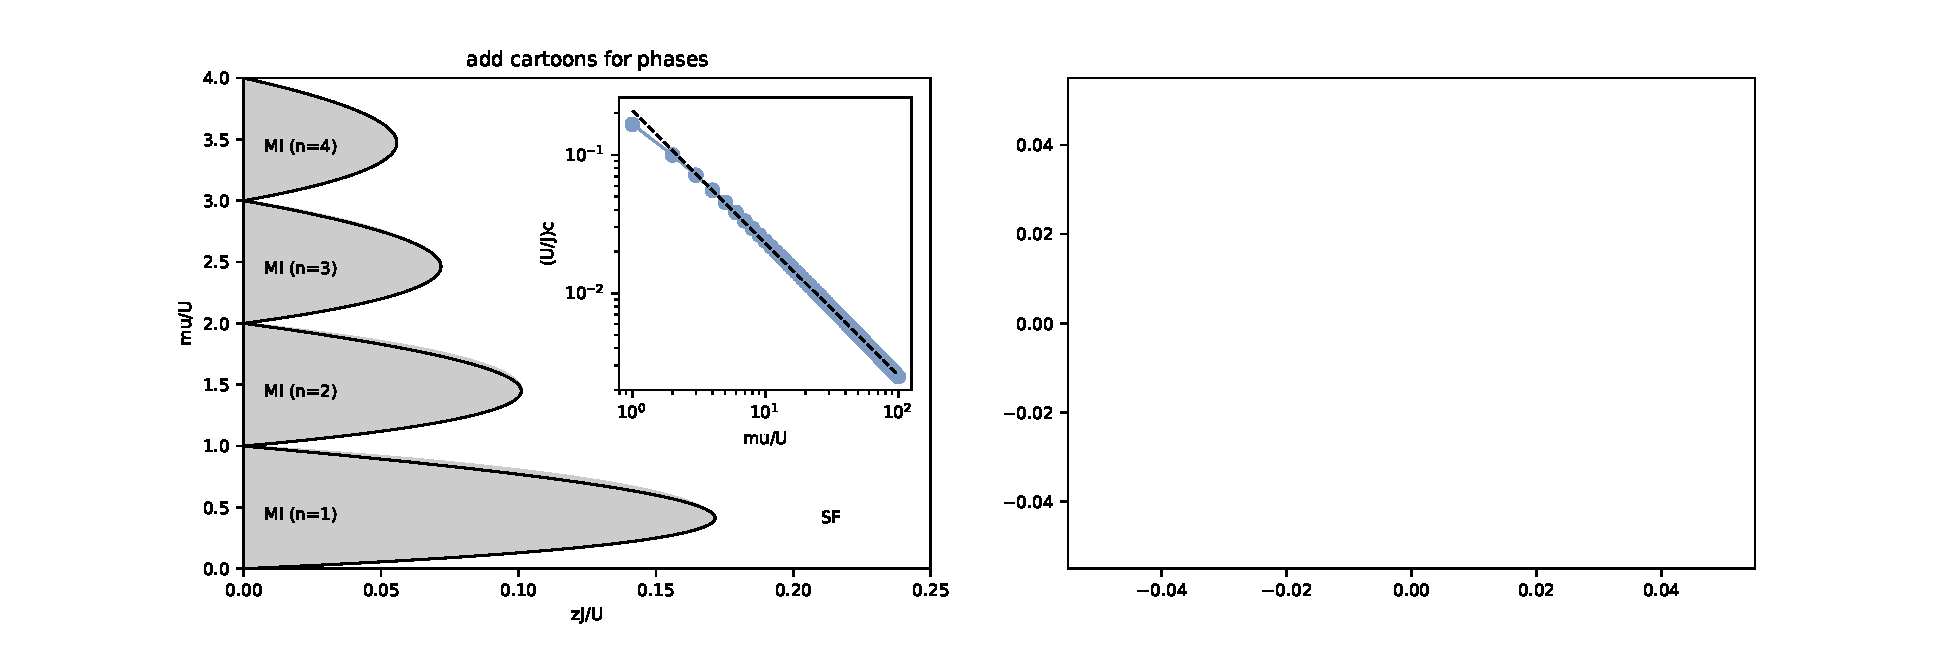
\includegraphics[width=\columnwidth]{figures/ch1/MeanFieldPhaseDiag/MeanFieldDiag.pdf} 
		\caption{\textbf{Mean-Field Phase Diagram. a,}  }
		\label{fig:MF}	
\end{figure}

It can be seen intuitively that the critical, finite value of ${U/J}_c$ depends on the on-site occupation number by comparing the kinetic energy scales to the gap in the system. We first start in a Mott-insulating plateau $|\Psi_{MI} \rangle$ with $n$ atoms per site which has a total energy of $E_0=L\cdot U n (n-1)$. The first excitation from this state involves moving an atom from site $i$ to its neighbor and has a total energy of $E_1 = (L-2) \cdot U n (n-1) + U(n+1)(n) + U(n-1)(n-2)$. The gap between these two states is given by $\Delta = E_1 - E_0 = U$ and notably is independent of the on-site occupation number $n$! Since the atoms are bosonic and identical, the kinetic energy term $J$ that connects these two states has a bosonic enhancement factor of $\sim n$ and means that the relevant comparison for distinguishing these two phases is $(U/J)_c \propto U/(n J)$. The peaks of the lobes in Fig.~\ref{fig:MF} and are plotted as a function of half integer chemical potential in the inset and agree with a power law exponent $n^{-1}$.


\section{Beyond flat, tight-binding Bose-Hubbard}

Bose-Glass?

off-site interaction, more than nearest neighbor tunneling, dipole moments?

Disorder effects on J and U cite De Marco, high-order tunneling, tilt and tunneling to higher bands

heating rates, probably refer to appendix




% For an example of a full page figure, see Fig.~\ref{fig:myFullPageFigure}.


%\texttt{This is a line of code.}






